%% BioMed_Central_Tex_Template_v1.06
%%                                      %
%  bmc_article.tex            ver: 1.06 %
%                                       %

%%IMPORTANT: do not delete the first line of this template
%%It must be present to enable the BMC Submission system to
%%recognise this template!!

%%%%%%%%%%%%%%%%%%%%%%%%%%%%%%%%%%%%%%%%%
%%                                     %%
%%  LaTeX template for BioMed Central  %%
%%     journal article submissions     %%
%%                                     %%
%%          <8 June 2012>              %%
%%                                     %%
%%                                     %%
%%%%%%%%%%%%%%%%%%%%%%%%%%%%%%%%%%%%%%%%%


%%%%%%%%%%%%%%%%%%%%%%%%%%%%%%%%%%%%%%%%%%%%%%%%%%%%%%%%%%%%%%%%%%%%%
%%                                                                 %%
%% For instructions on how to fill out this Tex template           %%
%% document please refer to Readme.html and the instructions for   %%
%% authors page on the biomed central website                      %%
%% http://www.biomedcentral.com/info/authors/                      %%
%%                                                                 %%
%% Please do not use \input{...} to include other tex files.       %%
%% Submit your LaTeX manuscript as one .tex document.              %%
%%                                                                 %%
%% All additional figures and files should be attached             %%
%% separately and not embedded in the \TeX\ document itself.       %%
%%                                                                 %%
%% BioMed Central currently use the MikTex distribution of         %%
%% TeX for Windows) of TeX and LaTeX.  This is available from      %%
%% http://www.miktex.org                                           %%
%%                                                                 %%
%%%%%%%%%%%%%%%%%%%%%%%%%%%%%%%%%%%%%%%%%%%%%%%%%%%%%%%%%%%%%%%%%%%%%

%%% additional documentclass options:
%  [doublespacing]
%  [linenumbers]   - put the line numbers on margins

%%% loading packages, author definitions

%\documentclass[twocolumn]{bmcart}
% uncomment this for twocolumn layout and comment line below
\documentclass{bmcart}

%%% Load packages
%\usepackage{amsthm,amsmath}
%\RequirePackage{natbib}
%\RequirePackage{hyperref}
\usepackage[utf8]{inputenc} %unicode support
\usepackage{graphicx}
\usepackage{tikz}
\usepackage{doi}
\usepackage{amsmath}
\usepackage{listings}
\usepackage{bera}
\usepackage{multirow}
%\usepackage[applemac]{inputenc} %applemac support if unicode package fails
%\usepackage[latin1]{inputenc} %UNIX support if unicode package fails
\lstdefinelanguage{json}{
    basicstyle=\normalfont\ttfamily,
    numbersep=8pt,
    showstringspaces=false,
    breaklines=true,
    frame=lines,
    backgroundcolor=\color{white},
}

%%%%%%%%%%%%%%%%%%%%%%%%%%%%%%%%%%%%%%%%%%%%%%%%%
%%                                             %%
%%  If you wish to display your graphics for   %%
%%  your own use using includegraphic or       %%
%%  includegraphics, then comment out the      %%
%%  following two lines of code.               %%
%%  NB: These line *must* be included when     %%
%%  submitting to BMC.                         %%
%%  All figure files must be submitted as      %%
%%  separate graphics through the BMC          %%
%%  submission process, not included in the    %%
%%  submitted article.                         %%
%%                                             %%
%%%%%%%%%%%%%%%%%%%%%%%%%%%%%%%%%%%%%%%%%%%%%%%%%


%\def\includegraphic{}
%\def\includegraphics{}



%%% Put your definitions there:
\startlocaldefs
\endlocaldefs


%%% Begin ...
\begin{document}

%%% Start of article front matter
\begin{frontmatter}

\begin{fmbox}
\dochead{Software}

%%%%%%%%%%%%%%%%%%%%%%%%%%%%%%%%%%%%%%%%%%%%%%
%%                                          %%
%% Enter the title of your article here     %%
%%                                          %%
%%%%%%%%%%%%%%%%%%%%%%%%%%%%%%%%%%%%%%%%%%%%%%

\title{gnparser: a Powerful Scientific Names Parser}

%%%%%%%%%%%%%%%%%%%%%%%%%%%%%%%%%%%%%%%%%%%%%%
%%                                          %%
%% Enter the authors here                   %%
%%                                          %%
%% Specify information, if available,       %%
%% in the form:                             %%
%%   <key>={<id1>,<id2>}                    %%
%%   <key>=                                 %%
%% Comment or delete the keys which are     %%
%% not used. Repeat \author command as much %%
%% as required.                             %%
%%                                          %%
%%%%%%%%%%%%%%%%%%%%%%%%%%%%%%%%%%%%%%%%%%%%%%

\author[
   addressref={aff1},
   corref={aff1},                       % id of corresponding address, if any
   email={dmozzherin@illinois.edu}
]{\inits{DYM}\fnm{Dmitry Y.} \snm{Mozzherin}}
\author[                  % id's of addresses, e.g. {aff1,aff2}
   noteref={n1},% id's of article notes, if any
   email={alexander.myltsev@phystech.edu}   % email address
]{\inits{AAM}\fnm{Alexander A.} \snm{Myltsev}}
\author[
   email={dpatterson.mbl@gmail.com}
]{\inits{DJP}\fnm{David J.} \snm{Patterson}}

%%%%%%%%%%%%%%%%%%%%%%%%%%%%%%%%%%%%%%%%%%%%%%
%%                                          %%
%% Enter the authors' addresses here        %%
%%                                          %%
%% Repeat \address commands as much as      %%
%% required.                                %%
%%                                          %%
%%%%%%%%%%%%%%%%%%%%%%%%%%%%%%%%%%%%%%%%%%%%%%

\address[id=aff1]{%                    % unique id
  \orgname{University of Illinois},    % university, etc
  \street{1816 South Oak St.},         %
  \city{Champaign},                    % city
  \state{IL},
  \postcode{61820},
  \cny{US}                             % country
}

%%%%%%%%%%%%%%%%%%%%%%%%%%%%%%%%%%%%%%%%%%%%%%
%%                                          %%
%% Enter short notes here                   %%
%%                                          %%
%% Short notes will be after addresses      %%
%% on first page.                           %%
%%                                          %%
%%%%%%%%%%%%%%%%%%%%%%%%%%%%%%%%%%%%%%%%%%%%%%

\begin{artnotes}
%\note{Sample of title note}     % note to the article
\note[id=n1]{Equal contributor} % note, connected to author
\end{artnotes}

\end{fmbox}% comment this for two column layout

%%%%%%%%%%%%%%%%%%%%%%%%%%%%%%%%%%%%%%%%%%%%%%
%%                                          %%
%% The Abstract begins here                 %%
%%                                          %%
%% Please refer to the Instructions for     %%
%% authors on http://www.biomedcentral.com  %%
%% and include the section headings         %%
%% accordingly for your article type.       %%
%%                                          %%
%%%%%%%%%%%%%%%%%%%%%%%%%%%%%%%%%%%%%%%%%%%%%%

\begin{abstractbox}

\begin{abstract} % abstract
  \parttitle{Background}
  Modern biology is unthinkable without names based on Linnaean nomenclature.
  Names of organisms are pervasive, they are metadata which allows to
  communicate information in biodiversity, ecology, molecular biology, medicine
  and many other fields. However indexing and organizing such information via
  scientific names is challenging for several reasons. As an example -- names
  exist in a variety of alternative forms like ``\textit{Aedes (Cancraedes)
  thurmanae}'' and ``\textit{Aedes thurmanae} Mattingly, 1958'', therefore a
  simple string comparison often fails to connect information via names due to
  these variations. Parsing would break names into semantic elements, allowing
  to compare them by their \textit{canonical form} (\textit{Aedes thurmanae}
  for both examples).
  \parttitle{Results}
  We introduce Global Names Parser (\textit{gnparser}) -- a tool based on
  Parsing Expression Grammar algorithm. The parser is able to deal with the
  most complex scientific name strings. It finds semantic meaning for all
  words within a scientific name (like ranks, years of publication, names of
  authors etc.). Global Names Parser is written in Scala, a Java Virtual
  Machine language.  Measured throughput was up to 20 million names/hour per
  CPU. Precision was X, Recall X, F-value X. We show that \textit{gnparser} is
  compatible with Scala, Java, R, Jython, and JRuby.
  \parttitle{Conclusions}
  Global Names Parser (\textit{gnparser}) is a long awaited tool for
  biodiversity informatics. It is released under Open Source MIT license. It
  allows to disassemble scientific names of any complexity into their semantic
  elements. It is scalable to deal with billions of name strings an hour, can
  be directly incorporated by many popular languages. The parser can be used as
  a command line application, socket server, or a web server.
\end{abstract}

%%%%%%%%%%%%%%%%%%%%%%%%%%%%%%%%%%%%%%%%%%%%%%
%%                                          %%
%% The keywords begin here                  %%
%%                                          %%
%% Put each keyword in separate \kwd{}.     %%
%%                                          %%
%%%%%%%%%%%%%%%%%%%%%%%%%%%%%%%%%%%%%%%%%%%%%%

\begin{keyword}
\kwd{biodiversity}
\kwd{scientific name}
\kwd{parser}
\end{keyword}

% MSC classifications codes, if any
%\begin{keyword}[class=AMS]
%\kwd[Primary ]{}
%\kwd{}
%\kwd[; secondary ]{}
%\end{keyword}

\end{abstractbox}
%
%\end{fmbox}% uncomment this for twcolumn layout

\end{frontmatter}

%%%%%%%%%%%%%%%%%%%%%%%%%%%%%%%%%%%%%%%%%%%%%%
%%                                          %%
%% The Main Body begins here                %%
%%                                          %%
%% Please refer to the instructions for     %%
%% authors on:                              %%
%% http://www.biomedcentral.com/info/authors%%
%% and include the section headings         %%
%% accordingly for your article type.       %%
%%                                          %%
%% See the Results and Discussion section   %%
%% for details on how to create sub-sections%%
%%                                          %%
%% use \cite{...} to cite references        %%
%%  \cite{koon} and                         %%
%%  \cite{oreg,khar,zvai,xjon,schn,pond}    %%
%%  \nocite{smith,marg,hunn,advi,koha,mouse}%%
%%                                          %%
%%%%%%%%%%%%%%%%%%%%%%%%%%%%%%%%%%%%%%%%%%%%%%

%%%%%%%%%%%%%%%%%%%%%%%%% start of article main body
% <put your article body there>

\section*{Conventions}

Throughout the paper we distinguish between two terms -- ``name'' and
``name-string''. Term ``name'' varies in its meaning for different
nomenclatural codes. According to botanical code of nomenclature \cite{ICN}
\textit{Pinus silvestris} is considered to be a single name. According to
zoological code \cite{ICZN} \textit{Parus major} is considered to be a
combination of two names -- \textit{Parus} and \textit{major}. In the paper we
use term ``name'' in ``botanical'' sense unless stated otherwise.

The ``name-string'' term represents a sequence of characters (letters, numbers,
punctuation, spaces, symbols) used to represent a name. Both \textit{Pinus
silvestris} and \textit{Parus major} correspond to one name-string each.

A name can be expressed by many name-strings, some are well-formed and code
compliant, and others are not (for example see Table~\ref{table:carex}). There
are millions of scientific names and billions of possible legitimate name
strings.

When we talk about ``code-compliancy'' we mean compliance with a corresponding
code of nomenclature (Zoological \cite{ICZN}, Botanical \cite{ICN},
Bacteria \cite{ICNB}, Viruses \cite{ICTV}, Cultivated plants \cite{ICNCP},
Phylocode \cite{ICPN}). Codes of nomenclature determine rules for composing
scientific names from infraspecific to family level. Other levels comply with
community practices.

\section*{Background}

The names of organisms are invaluable in the world of big biodiversity data
because they can be used as near universal metadata to index, organize and
interconnect distributed information \cite{Patterson2010}. Nevertheless, use of
names for informatics purposes presents an array of problems. As we demonstrate
further many of these problems can be solved by parsing, or deducing the
semantic meaning of words occurred in the name-strings.

\begin{table}[!htb]
  \begin{center}

  \caption{Some legitimate versions of the scientific name for the Northern
    Bulrush or Singlespike sedge.  The genus (Carex), species (scirpoidea),
    and subspecies (convoluta) may be annotated (var. subsp., and ssp.) or
    have the name of the original authority for the infraspecies (Kükenthal),
    the species (Michaux), the current infraspecific combination (Dunlop),
    sometimes abbreviated and with or without dates. Image courtesy of
  \cite{FNA2002}.}\label{table:carex}

    \begin{tabular}{| l | c |}
    \hline
    Carex scirpoidea convoluta &
    \multirow{24}{*}{\includegraphics[scale=0.3]{images/carex.png}} \\
    Carex scirpoidea var. convoluta & \\
    Carex scirpoidea subsp. convoluta & \\
    Carex scirpoidea convoluta Kükenth. & \\
    Carex scirpoidea var. convoluta Kuk. & \\
    Carex scirpoidea var. convoluta Kük. & \\
    Carex scirpoidea var. convoluta Kükenth. & \\
    Carex scirpoidea var. convoluta Kükenthal & \\
    Carex scirpoidea Michx. var. convoluta Kük. & \\
    Carex scirpoidea ssp. convoluta (Kük.) Dunlop & \\
    Carex scirpoidea Michx. var. convoluta Kükenth. & \\
    Carex scirpoidea subsp. convoluta (Kük.) Dunlop & \\
    Carex scirpoidea ssp. convoluta (Kukenth.) Dunlop & \\
    Carex scirpoidea Michaux var. convoluta Kükenthal & \\
    Carex scirpoidea subsp. convoluta (Kük.) D.A.Dunlop & \\
    Carex scirpoidea subsp. convoluta (Kük.) D.A. Dunlop & \\
    Carex scirpoidea Michx. ssp. convoluta (Kük.) Dunlop & \\
    Carex scirpoidea subsp. convoluta (Kuk.) D. A. Dunlop & \\
    Carex scirpoidea Michx. subsp. convoluta (Kük.) Dunlop & \\
    Carex scirpoidea Michx. ssp. convoluta (Kükenth.) Dunlop & \\
    Carex scirpoidea subsp. convoluta (Kükenthal) D.A. Dunlop & \\
    Carex scirpoidea Michx. subsp. convoluta (Kük.) D.A.Dunlop & \\
    Carex scirpoidea Michx. subsp. convoluta (Kük.) D.A. Dunlop & \\
    Carex scirpoidea subsp. convoluta (Kükenthal 1909) D.A. Dunlop 1998 & \\
    \hline
    \end{tabular}
  \end{center}
\end{table}

Due to intrinsic diversity of name-strings (Table~\ref{table:carex}) an exact
string matching is not powerful enough to link distributed big data via
scientific names. This problem can be addressed by promoting a rigid standard
restricting each name to a single name-string, or through
\textit{reconciliation}. The former strategy would require a costly
international coordination, would not eliminate future human mistakes, it
cannot be applied to older documents, does not allow for multiple points of
view, nor for changes in taxonomic perspective.

The reconciliation process involves folding of all known name-strings into
lexical groups. This requires that we collate all variant spellings of names.
Parsing in crucial for creating lexical groups of name-strings: it allows to
find the most common denominator of spelling variants -- a canonical form
(\textit{Carex scirpoidea convoluta} in case of Table~\ref{table:carex}) and
extract other important for reconciliation  information (infraspecific ranks,
original and combination authorities etc.). Lexical groups would then require
another level of folding into reconciliation groups where homotypic and
heterotypic synonyms are placed together. This process requires an accurate
database of nomenclatural events (for example Global Names Usage Bank
\cite{Pyle2003}).

Reconciliation uses the most stable component of a name-string -- its canonical
form. Such approach brings us to another problem -- the same canonical form may
be used for more than one taxon or concept in case of homonyms, chresonyms, or
ranks of infraspecies. Analysis of ranks and the authors found by a
parser in name-strings helps to separate homonyms and similar names from each
other.

The next challenge is to replace outdated names with ones that are endorsed by
taxonomic authorities -- this is a process referred to as \textit{resolution}.
Resolution requires an up to date high quality taxonomic and nomenclatural data
to map a reconciled name-string to the currently used name/names. A
reconciliation of name-strings used by a taxonomic authority with name-strings
supplied by user makes parsing a very important step at this stage as well.

A significant number of biodiversity informatics projects (Encyclopedia of Life
\cite{eol}, Global Biodiversity Informatics Facility \cite{gbif}, Catalogue of
Life \cite{col}, World Register of Marine Species \cite{worms}, iDigBio
\cite{idigbio}, VertNet \cite{vertnet} etc.) aggregate information from many
different sources.  Resulting name-strings are inconsistent in their format.
Parsed names can be normalized to the same style. Some name strings are not
properly formed, other contain annotations which are not part of the name.
There are also “surrogate names” -- they depict organisms which were not fully
identified and mapped to a formally described taxon, instead they were
associated with a name string that narrows down identification choices to some
higher clade. Parser helps to recognize such names and mark them as surrogate
name-strings.

After collecting parsed data from a large name-string repository a researcher
can use the data as a basis for statistical analysis, or for practical
purposes. For example parsed data can be used to introduce faceted search by
authors name, year of publication, species epithet etc. If a name-string cannot
be ingested by a high quality parser, the string is almost certainly not a
well-formed scientific name. As a result parser can weed out problematic name
strings from collection.

\subsection*{Prior Art}

Until recently the problem of scientific name parsing had been addressed by
home-grown scripts running regular expressions or by manual splitting of a name
into its canonical form and the authorship part. Both approaches proved to be
limited. Regular expressions are not designed for recursive patterns (and
complex scientific name strings are recursive by nature, as it is most obvious
with hybrid formulae). Manual approach of splitting names into 2 parts is
expensive, slow, inflexible and cannot elegantly deal with name-strings where
authorship is present in the middle of the name.

Names can be quite complex (for example ``\textit{Brassica oleracea} L.
\textit{subsp.  capitata} (L.) DC. \textit{convar. fruticosa} (Metzg.) Alef.
$\times$ \textit{B. oleracea} L.  \textit{subsp. capitata} (L.) \textit{var.
costata} DC.'')  and include authorship for every mentioned taxon, include or
omit infraspecific ranks, original and combination authors etc. Authorship
itself is quite complex and can include original authors who described a name,
authors of a new combination, or authors who made a name, but did not publish
it. We obviously do not want to exclude names from biodiversity informatics
just because they are not simple enough. We need an approach that is able to
deal with names of any complexity.

In 2008 we decided to create a specialized parsing library
``\textit{biodiversity}'' \cite{biodiversity} written in Ruby and based on
Parsing Expression Grammar (PEG) methodology \cite{Ford2004}. We used an
excellent TreeTop Ruby library \cite{treetop} as an underlying PEG
implementation. PEG is well suited for recursive texts with formally defined
grammars. Scientific names follow rules of nomenclatural codes, and therefore
order and capitalization of elements in scientific names are well structured.

We found that PEG approach allows us to solve all these complexity gracefully.
Also PEG gave us enough flexibility to incorporate edge cases and common
mistakes in formation of names. The library \textit{biodiversity} enjoyed
noticeable popularity. At the time of writing it had been downloaded more than
150,000 times \cite{bdiv_downloads}, it is used by many taxon name resolution
projects (for example by Canadian Register of Marine Species (CARMS)
\cite{carms}, the iPlant TNRS \cite{iplant}, World Registry of Marine Species
(WoRMS) \cite{worms}.  According to BioRuby statistics \textit{biodiversity}
parser is the most popular bio-library in Ruby language \cite{biogems}.

We consider \textit{biodiversity} parser library to be a working prototype -- a
playground which allowed us to identify parsing problems and implement
solutions for them. In the process we found that Parsing Expression Grammar is
very well suited for breaking scientific names into semantic elements. In 2015
we decided to use everything we learned and write ``\textit{gnparser}'' a
completely new parser in Scala to achieve significant boost in speed,
scalability and portability of the library. In this manuscript we describe
features, performance and discuss future enhancements of this new parser.

\section*{Implementation}

- existing language classes: regular languages, Deterministic context-free languages, Parsing expression grammars, General context-free. Why PEGs?

- existing implementations of PEG parser generator % https://en.wikipedia.org/wiki/Comparison_of_parser_generators}

- existing combinator parsers. written in parboiled2/Scala. What was the reason for the choice?

- gnparser consists of three parts. Short description of parts

\subsection*{Parser}

- explanation of functionality: parser engine

- dependency of the rest 2 components on this one

- versions of scala supported

- relation to biodiversity parserj

- relationship to parboiled2, mention Alex' role in paraboiled2

- patches to parboiled2 (+ links to human-readable explanation: blog or published paper)

- bottlenecks optimizations in parser

- input: name string(s), output: JSON object.

- Figure with output example and short explanation

- Quality output -- short explanation.

- reference to JSON schema (attachment), simple explanation of fields
(attachment)

- short explanations of tests. Connection between tests and schema

- usage with other languages as a library

\subsection*{Runner}

- explanation of functionalilty: command line tool, socket server

- command line tool -- input for one name, output, intput for file, output

- socket server -- very short explanation how it runs. Input, Output

- mention parallelization in parsing

- TODO: should we change input output to be more similar to REST API?
  Make it JSON array of names as input, array of gnparser objects as output

\subsection*{Web}

- explanation of functionality: Web GUI, REST API

- input and output for API use via GET and POST

\subsection*{Installation}

- reference to README. Reference and short explanation of the Docker project
(in attachments)

- MIT license

\subsection*{Testing Methods}

Data for our tests were name-strings randomly chosen from 24 million
name-strings of the Global Names Index. These resulting datasets consisted of
strings acquired from a variety of data sources and were a mixture of
well-formed names, names with formatting and spelling mistakes, and non-name
strings misrepresented as names.

We compared performance of gnparser with 2 other projects -- Biodiversity
parser\cite{biodiversity} (also developed by Global Names), and GBIF
name-parser\cite{gbifNameParser}. Another project we considered was YASMEEN
parser from iMarine\cite{VandenBerghe2015}, however we found that with our
dataset it generated dramatically more mistakes than other parsers
($Precision$ 0.534, $Recall$ 1.0, $F1$ 0.6962), and we decided to exclude it
from the tests.

To find out the throughput of parsing we used a computer with Intel i7-4930K
CPU (6 cores, 12 threads, at 3.4 GHz), 64GB of memory, and 250GB Samsung 840
EVO SSD, running Ubuntu version 14.04. Throughput was determined by processing
1,000,000 name-strings.

To study effects of parallel execution on throughput we used
\textit{ParallelParser} class from Biodiversity parser and \textit{gnparse}
command line interface for gnparser. For GBIF name-parser we created a thin
wrapper with multi-threaded capabilities\cite{gbifparser}.

For determining $Precision$, $Recall$ and $Accuracy$ of parsed names the
dataset size was 1000 name-strings. To estimate quality for all parsers we
needed to pick a feature which is common for all three of them and is a good
indicator of performance.  We decided to use a combination of canonical form
and terminal authorship.  Canonical form represents the most stable elements
of a name, while terminal authorship corresponds to the authority of the most
detailed element of the name. For example in "\textit{Oriastrum lycopodioides}
Wedd.  var.  \textit{glabriusculum} Reiche" canonical form is
"\textit{Oriastrum lycopodioides glabriusculum}" and terminal authorship is
"Reiche", not "Wedd.".  Algorithms necessary to select components of a
canonical form of a name and to find the terminal authorship are good
indicators of a parser quality.

When both the canonical form and the terminal authorship were determined
correctly we marked the result as true positive ($\text{tp}$).  If one or both
of them were determined incorrectly -- the result was marked a false positive
($\text{fp}$). Correctly discarded from parsing name-strings were marked as
true negatives ($\text{tn}$). False negatives ($\text{fn}$) were "suitable"
name-strings which should be parsed, but were nevertheless discarded.

Some names in the dataset were not well-formed. If a human could extract the
canonical form and the terminal authorship from them we did count them.
Examples of such name-strings are \textbf{"Bumetopia (bumetopia)
quadripunctata Breuning"} (low case subgenus), \textbf{"Campylium gollanii C.
M?ller ex Vohra 1970 [1972]"} (miscoded UTF-8 symbol and additional year in
square brackets), \textbf{"Myosorex muricauda (Miller, 1900)."} (period after
authorship).

$Precision$ is a percentage of names parsed correctly and is calculated as

\[Precision = \dfrac{\text{tp}}{(\text{tp} + \text{fp})}\]

$Recall$ is a percentage of names detected and is calculated as

\[Recall = \dfrac{\text{tp}}{(\text{tp} + \text{fn})}\]

$F1-measure$ is a balanced harmonic mean (where $Precision$ and $Recall$ have
the same weight). When both $Precision$ and $Recall$ vary, $F1-measure$ allows
to compare results nevertheless. It is calculated as

\[F1 = \dfrac{2 \times Precision \times Recall}{(Precision + Recall)}\]

$Accuracy$ is a pecentage of correct results. It is calculated as

\[Accuracy = \dfrac{\text{tp} + \text{tn}}
  {\text{tp} + \text{tn} + \text{fp} + \text{fn}}\]

Validity of names was not taken into account, as it is out of scope of
parsers' functionality. For example in case of a name-string \textbf{"Example
name Word var.  something Capitalized Words, 1900"}, canonical form
\textbf{"Example name something"} and terminal authorship \textbf{"Capitalized
Words, 1900"} would be considered a true positive.

It is important for parser to accurately distinguish between strings of
scientific names, names of viruses, surrogate names, and non-names. To find
out how well parsers distinguished strings which are not scientific names, we
calculated $Precision$ for discarded/non-parsed strings. If done correctly
not-parsed strings would include only names of viruses and non-scientific
names.

We processed 100,000 name-strings by each parser, and about 1000 of them had
been discarded as not-parseable. $Precision$ in this case showed percentage of
correctly discarded names.  We do not know $Recall$, as it was not feasible to
manually find it for 100 000 names. To get a glimpse on names which had to be
discarded, but were parsed instead we analysed intersections and differences
of the results between the three parsers.

\section*{Results and Discussion}

The goal of Global Names Architecture is to create an infrastructure for
biology which uses scientific names to connect and inter-exchange biological
data in the most complete and painless way. Parsing is the first step to this
goal. What are requirements for a parser to be suitable for such a task?

1. \textbf{High Quality}. Parser should be able to break names into their
semantic elements as good or better than a human. If we able to reach this
goal we become independent on how names are stored in various databases. We
will not be limited to sources with already preparsed names. Moreover, we hope
to make obsolete a very expensive step of humans prepasing names by the
advent of accessible high quality parsers.

2. \textbf{Global Scope}. Parser should be able to support all types of
scientific names, including the most complex ones like hybrid formulas,
multi-infraspecific names, names with nested authorships etc. Without parsing
ability to find the same name in different sources is severely diminished
and for unparsed names it will mean that information attached to them will be
hidden from the eyes of the researchers.

3. \textbf{Parsing Completeness}. All information indluded into a name is
important, not only canonical form. Authorship, year, rank information allows
to distinguish homonyms, synonyms, spelling mistakes, chresonyms from each
other, narrow search down to relevant information. From other side it allows
people who manage large collections of names to weed out mistakes and
increase quality of their databases.

4. \textbf{Speed}. If Global Names serves its goal well it will need to be
very fast and effective to satisfy needs of users everywhere on the globe.
High throughput of parsing becomes very important and from one side it
increases speed with which people will receive requested information, from
other side it directly influences the cost of required hardware, as well as
the cost of hardware upgrades.

5. \textbf{Accessibility}. We think it is important to make parsing ubiquitos
and accessible to everyone. It should be assessible as a library, as a command
line tool, as a desktop or GUI program. It should be easy to use, easy to
install. As a library it has to be usable in many languages. It should have

In further text we are going to talk about gnparser from the point of these 5
requirements

\subsection*{High quality parsing}

High quality parsing is probaby the most important of the 5 requirements. We
tested gnparser together with 3 other parsing projects. To our knowledge these
three represent the state of the art for parsing biological names. GBIF parser
uses regular expressions approach and gnparser and biodiversity parser use PEG
approach.

Results for our quality measurements are shown in Table~\ref{table:precision}.
With datasets where true negatives ($\text{tn}$) create a large proportion of
data $Accuracy$ is not a good measure, as it would favor algorithms which
distinquish negative results rather than finding positive ones. However in our
case true negatives are rare and have a very little influence. We can also see
that $Recal$ for all parsers was very high, which means false negatives had
almost no influence on results as well. Taking this in account we think
$Accuracy$ is the best measure for our tests and alone is sufficient to
compare quality for all cases.

Altogether we find that all 3 parsers performed very well with our tests
showing $Accuracy \textgreater 95\%$ while gnparser and biodiversity parser
approaching 99\% mark. Moreover, most of the false positives came from names
with mistakes. For example, out of 11 false positives for gnparser only 2 were
well-formed names:

\begin{verbatim}
    Eucalyptus subser. Regulares Brooker
    Jacquemontia spiciflora (Choisy) Hall. fil.

    Acanthocephala declivis variety guianensis Osborn, 1904
    Atysa (?) frontalis
    Bumetopia (bumetopia) quadripunctata Breuning, 1950
    Cyclotella kã¼tzingiana Thwaites
    Elaphidion (romaleum) tæniatum Leconte, 1873
    Hieracium nobile subsp. perclusum (Arv. -Touv. ) O. Bolòs & Vigo
    Leptomitus vitreus (Roth) Agardh{?}
    Myosorex muricauda (Miller, 1900).
    Papillaria amblyacis (M<81>ll.Hal.) A.Jaeger
\end{verbatim}

When parsers reach close to 90\% accuracy they hit a "long tail" of problems
where each particular case of wrong parsing is rare, and every new random test
reveals new problems. Good thing that for all 3 parsers developer teams
performed this meticulous work adding one rare case after another to the list
of problems and finding ways to incoporate solutions. Quality of parsing rules
is constantly improving, and we belive reaching  $Accuracy \textgreater
99.5\%$ reliably is achievable with PEG parsers.

During incorporation of new rules and increasing $Recall$ it is important to
judge if a problem has a potential of bringing down $Precision$ by introducing
new false positives.  For example GBIF name-parser allows genus of a
name-string to be in a lowcase. As a restult the strings below got parsed as
scientific names, while other parsers ignored them:


\begin{verbatim}
    acid mine drainage metagenome
    agricultural soil bacterium CRS5639T18-1
    agricultural soil bacterium SC-I-8
    algal symbiont of Cladonia variegata MN075
    alpha proteobacterium AP-24
    anaerobic bacterium ANA No.5
    anoxygenic photosynthetic bacterium G16
    archaeon enrichment culture clone AOM-SR-A23
    bacterium endosymbiont of Plateumaris fulvipes
    bacterium enrichment culture DGGE band 61_3_FG_L
    barley rhizosphere bacterium JJ-220
    bovine rumen bacterium niuO17
\end{verbatim}

Solutions like these significantly increase $Recall$ for certain low-quality
datasets, but as we see in this example they also bring risk to precipitously
decrease $Precision$ with other datasets as we found out in case of YASMEEN
iMarine parser.

We think that in cases like this to write parsers carefully considering every
case of increased $Recall$ and investigate what kind of problems it might
bring to $Precision$. If parser is written for a very specific "dirty" dataset
it might be appropriate to deviate singificantly from adopted nomenclatural
rules. In our case we want to write a \textbf{generic} parser suitable for
majority of users. If such users do have a "dirty" dataset with very
predictable problems (like lowcase genus) we recommend to write a preparser
script which "normalizes" known problems and then use a high quality parser.

Our testing also revealed differences between regular expressions approach and
PEG approaches. Our results show that both appraches can achieve high quality,
but regular expressions approach hits the ceiling faster. The reason for this
is recursive nature of scientific names. It is much easier to cover simpler
structured (probably ~80\%) of scientific names with regular expression, than
with PEG, but after easy part is done complications arising from recursive
nature of names arise until they become unsurmantable.

\subsection*{Global Scope}

If we want to trully connect biological data using scientific names, no names
should be left behind, no matter how complex they are. We use PEG approach to
parsing because it allows to nest parsing rules within each other, making it
possible to create progressively more and more comples rules. The first rule
just defines what space is, the last rule defines hybrid formula. Regular
expressions do not support recursion as a result the more complex name is the
harder it becomes to support them.

During out testing we found that $Accuracy$ of GBIF parser was negatively
affected by inability to parse hybrid formulas and incorrect parsing of
infrasubspecies names (names with more then one infraspecific epithet). For
example:

\begin{verbatim}
    Crataegus chlorosarca subtaxon pubescens E.L.Wolf
    Erigeron peregrinus ssp.callianthemus var. eucallianthemus
    Salvelinus fontinalis x Salmo gairdneri
    Echinocereus fasciculatus var. bonkerae × E. fasciculatus var. fasciculatus
\end{verbatim}

We have to support names like this, and PEG parsers allow us do do that.


\begin{table}[htb]
  \begin{center}
    \caption{Precision/Recall for processed by parsers 1000
    name-strings}\label{table:precision}
    \begin{tabular}{|l|*{3}{l}|}
      \hline
                             & gnparser & gbif-parser & biodiversity \\
      \hline
      \textit{True Positive} & 976      & 955         & 971          \\
      \textit{True Negative} & 13       & 12          & 13           \\
      \textit{False Positive}& 11       & 32          & 16           \\
      \textit{False Negative}& 0        & 1           & 0            \\
      \textit{Precision}     & 0.9888551& 0.967578    & 0.9837893    \\
      \textit{Recall}        & 1.0      & 0.998954    & 1.0          \\
      \textit{F1}            & 0.9943963& 0.983016    & 0.9918284    \\
      \textit{Accuracy}      & 0.989    & 0.967       & 0.984        \\
      \hline
    \end{tabular}
  \end{center}
\end{table}

\begin{table}[htb]
  \begin{center}
    \caption{Precision for discarded by parsers names, out of 100 000
    name-strings}\label{table:unparsed}
    \begin{tabular}{|l|*{3}{l}|}
      \hline
                              & gnparser & gbif-parser & biodiversity \\
      \hline
      \textit{Total discarded}& 1131     & 1082        & 1161         \\
      \textit{True Positive}  & 1129     & 940         & 1152         \\
      \textit{False Positive} & 2        & 142         & 9            \\
      \textit{Precision}      & 0.998231 & 0.868761    & 0.9922481    \\
      \hline
    \end{tabular}
  \end{center}
\end{table}

\begin{figure}[htbp]
  \begin{center}
    \caption{
      Names parsed per second by GN, GBIF and Biodiversity parsers
      (runing on 1-12 parallel threads).
    }\label{figure:throughput}
    \vspace{0.5cm}
    \begin{tabular}{| l | *{3}{r} | c c c |}
      \hline
      \multirow{1}{*}Threads & gnparser & gbif-paser & biodiversity
      & \multicolumn{3}{c |}{Ratio} \\
      \cline{5-7}
      & & & & gn & gbif & bio \\
      \hline
      1  & 5944  & 6389  & 1111 & 1 & 1.07 & 0.19 \\
      2  & 11416 & 12638 & 1722 & 1 & 1.11 & 0.14 \\
      4  & 20500 & 21994 & 2556 & 1 & 1.07 & 0.12 \\
      8  & 24805 & 30972 & 2777 & 1 & 1.25 & 0.11 \\
      12 & 26055 & 31833 & 2527 & 1 & 1.22 & 0.10 \\
      \hline
    \end{tabular}
    % Created by tikzDevice version 0.10.1 on 2016-06-02 07:38:12
% !TEX encoding = UTF-8 Unicode
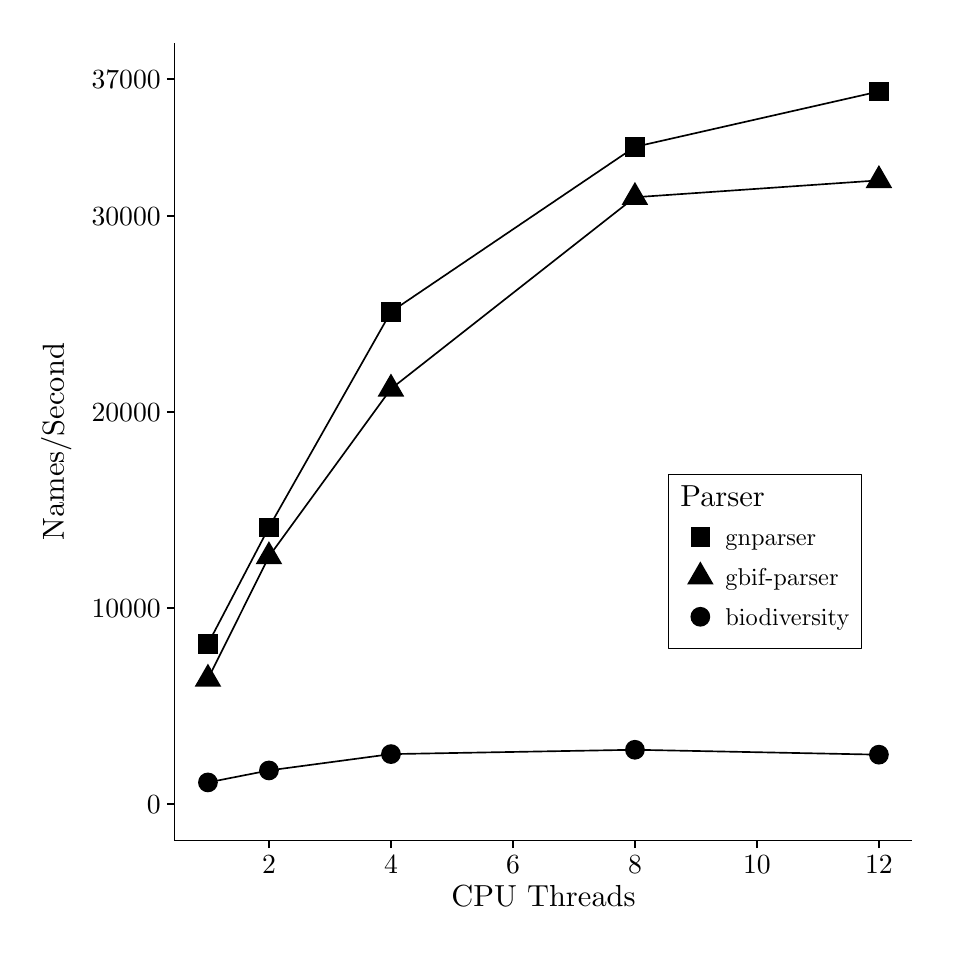
\begin{tikzpicture}[x=1pt,y=1pt]
\definecolor{fillColor}{RGB}{255,255,255}
\path[use as bounding box,fill=fillColor,fill opacity=0.00] (0,0) rectangle (325.21,325.21);
\begin{scope}
\path[clip] (  0.00,  0.00) rectangle (325.21,325.21);
\definecolor{drawColor}{RGB}{255,255,255}
\definecolor{fillColor}{RGB}{255,255,255}

\path[draw=drawColor,line width= 0.6pt,line join=round,line cap=round,fill=fillColor] (  0.00,  0.00) rectangle (325.21,325.21);
\end{scope}
\begin{scope}
\path[clip] ( 53.02, 31.51) rectangle (319.71,319.71);
\definecolor{fillColor}{RGB}{255,255,255}

\path[fill=fillColor] ( 53.02, 31.51) rectangle (319.71,319.71);
\definecolor{drawColor}{RGB}{255,255,255}

\path[draw=drawColor,line width= 0.3pt,line join=round] ( 53.02, 80.02) --
	(319.71, 80.02);

\path[draw=drawColor,line width= 0.3pt,line join=round] ( 53.02,150.83) --
	(319.71,150.83);

\path[draw=drawColor,line width= 0.3pt,line join=round] ( 53.02,221.64) --
	(319.71,221.64);

\path[draw=drawColor,line width= 0.3pt,line join=round] ( 53.02,281.83) --
	(319.71,281.83);

\path[draw=drawColor,line width= 0.3pt,line join=round] ( 65.14, 31.51) --
	( 65.14,319.71);

\path[draw=drawColor,line width= 0.3pt,line join=round] (109.22, 31.51) --
	(109.22,319.71);

\path[draw=drawColor,line width= 0.3pt,line join=round] (153.31, 31.51) --
	(153.31,319.71);

\path[draw=drawColor,line width= 0.3pt,line join=round] (197.39, 31.51) --
	(197.39,319.71);

\path[draw=drawColor,line width= 0.3pt,line join=round] (241.47, 31.51) --
	(241.47,319.71);

\path[draw=drawColor,line width= 0.3pt,line join=round] (285.55, 31.51) --
	(285.55,319.71);

\path[draw=drawColor,line width= 0.6pt,line join=round] ( 53.02, 44.61) --
	(319.71, 44.61);

\path[draw=drawColor,line width= 0.6pt,line join=round] ( 53.02,115.42) --
	(319.71,115.42);

\path[draw=drawColor,line width= 0.6pt,line join=round] ( 53.02,186.24) --
	(319.71,186.24);

\path[draw=drawColor,line width= 0.6pt,line join=round] ( 53.02,257.05) --
	(319.71,257.05);

\path[draw=drawColor,line width= 0.6pt,line join=round] ( 53.02,306.61) --
	(319.71,306.61);

\path[draw=drawColor,line width= 0.6pt,line join=round] ( 87.18, 31.51) --
	( 87.18,319.71);

\path[draw=drawColor,line width= 0.6pt,line join=round] (131.27, 31.51) --
	(131.27,319.71);

\path[draw=drawColor,line width= 0.6pt,line join=round] (175.35, 31.51) --
	(175.35,319.71);

\path[draw=drawColor,line width= 0.6pt,line join=round] (219.43, 31.51) --
	(219.43,319.71);

\path[draw=drawColor,line width= 0.6pt,line join=round] (263.51, 31.51) --
	(263.51,319.71);

\path[draw=drawColor,line width= 0.6pt,line join=round] (307.59, 31.51) --
	(307.59,319.71);
\definecolor{drawColor}{RGB}{0,0,0}

\path[draw=drawColor,line width= 0.6pt,line join=round] ( 65.14, 52.48) --
	( 87.18, 56.81) --
	(131.27, 62.71) --
	(219.43, 64.28) --
	(307.59, 62.51);

\path[draw=drawColor,line width= 0.6pt,line join=round] ( 65.14, 89.85) --
	( 87.18,134.11) --
	(131.27,194.69) --
	(219.43,263.93) --
	(307.59,270.03);

\path[draw=drawColor,line width= 0.6pt,line join=round] ( 65.14,102.52) --
	( 87.18,144.63) --
	(131.27,222.53) --
	(219.43,282.13) --
	(307.59,302.15);
\definecolor{fillColor}{RGB}{0,0,0}

\path[fill=fillColor] ( 61.57, 98.95) --
	( 68.71, 98.95) --
	( 68.71,106.09) --
	( 61.57,106.09) --
	cycle;

\path[fill=fillColor] ( 83.61,141.07) --
	( 90.75,141.07) --
	( 90.75,148.20) --
	( 83.61,148.20) --
	cycle;

\path[fill=fillColor] (127.70,218.96) --
	(134.83,218.96) --
	(134.83,226.10) --
	(127.70,226.10) --
	cycle;

\path[fill=fillColor] (215.86,278.56) --
	(223.00,278.56) --
	(223.00,285.69) --
	(215.86,285.69) --
	cycle;

\path[fill=fillColor] (304.02,298.58) --
	(311.16,298.58) --
	(311.16,305.72) --
	(304.02,305.72) --
	cycle;

\path[fill=fillColor] ( 65.14, 95.40) --
	( 69.95, 87.08) --
	( 60.34, 87.08) --
	cycle;

\path[fill=fillColor] ( 87.18,139.66) --
	( 91.99,131.34) --
	( 82.38,131.34) --
	cycle;

\path[fill=fillColor] (131.27,200.24) --
	(136.07,191.92) --
	(126.46,191.92) --
	cycle;

\path[fill=fillColor] (219.43,269.48) --
	(224.23,261.16) --
	(214.62,261.16) --
	cycle;

\path[fill=fillColor] (307.59,275.58) --
	(312.40,267.25) --
	(302.79,267.25) --
	cycle;

\path[fill=fillColor] ( 65.14, 52.48) circle (  3.57);

\path[fill=fillColor] ( 87.18, 56.81) circle (  3.57);

\path[fill=fillColor] (131.27, 62.71) circle (  3.57);

\path[fill=fillColor] (219.43, 64.28) circle (  3.57);

\path[fill=fillColor] (307.59, 62.51) circle (  3.57);
\end{scope}
\begin{scope}
\path[clip] (  0.00,  0.00) rectangle (325.21,325.21);
\definecolor{drawColor}{RGB}{0,0,0}

\path[draw=drawColor,line width= 0.6pt,line join=round] ( 53.02, 31.51) --
	( 53.02,319.71);
\end{scope}
\begin{scope}
\path[clip] (  0.00,  0.00) rectangle (325.21,325.21);
\definecolor{drawColor}{RGB}{0,0,0}

\node[text=drawColor,anchor=base east,inner sep=0pt, outer sep=0pt, scale=  1.00] at ( 48.07, 41.17) {0};

\node[text=drawColor,anchor=base east,inner sep=0pt, outer sep=0pt, scale=  1.00] at ( 48.07,111.98) {10000};

\node[text=drawColor,anchor=base east,inner sep=0pt, outer sep=0pt, scale=  1.00] at ( 48.07,182.79) {20000};

\node[text=drawColor,anchor=base east,inner sep=0pt, outer sep=0pt, scale=  1.00] at ( 48.07,253.60) {30000};

\node[text=drawColor,anchor=base east,inner sep=0pt, outer sep=0pt, scale=  1.00] at ( 48.07,303.17) {37000};
\end{scope}
\begin{scope}
\path[clip] (  0.00,  0.00) rectangle (325.21,325.21);
\definecolor{drawColor}{RGB}{0,0,0}

\path[draw=drawColor,line width= 0.6pt,line join=round] ( 50.27, 44.61) --
	( 53.02, 44.61);

\path[draw=drawColor,line width= 0.6pt,line join=round] ( 50.27,115.42) --
	( 53.02,115.42);

\path[draw=drawColor,line width= 0.6pt,line join=round] ( 50.27,186.24) --
	( 53.02,186.24);

\path[draw=drawColor,line width= 0.6pt,line join=round] ( 50.27,257.05) --
	( 53.02,257.05);

\path[draw=drawColor,line width= 0.6pt,line join=round] ( 50.27,306.61) --
	( 53.02,306.61);
\end{scope}
\begin{scope}
\path[clip] (  0.00,  0.00) rectangle (325.21,325.21);
\definecolor{drawColor}{RGB}{0,0,0}

\path[draw=drawColor,line width= 0.6pt,line join=round] ( 53.02, 31.51) --
	(319.71, 31.51);
\end{scope}
\begin{scope}
\path[clip] (  0.00,  0.00) rectangle (325.21,325.21);
\definecolor{drawColor}{RGB}{0,0,0}

\path[draw=drawColor,line width= 0.6pt,line join=round] ( 87.18, 28.76) --
	( 87.18, 31.51);

\path[draw=drawColor,line width= 0.6pt,line join=round] (131.27, 28.76) --
	(131.27, 31.51);

\path[draw=drawColor,line width= 0.6pt,line join=round] (175.35, 28.76) --
	(175.35, 31.51);

\path[draw=drawColor,line width= 0.6pt,line join=round] (219.43, 28.76) --
	(219.43, 31.51);

\path[draw=drawColor,line width= 0.6pt,line join=round] (263.51, 28.76) --
	(263.51, 31.51);

\path[draw=drawColor,line width= 0.6pt,line join=round] (307.59, 28.76) --
	(307.59, 31.51);
\end{scope}
\begin{scope}
\path[clip] (  0.00,  0.00) rectangle (325.21,325.21);
\definecolor{drawColor}{RGB}{0,0,0}

\node[text=drawColor,anchor=base,inner sep=0pt, outer sep=0pt, scale=  1.00] at ( 87.18, 19.68) {2};

\node[text=drawColor,anchor=base,inner sep=0pt, outer sep=0pt, scale=  1.00] at (131.27, 19.68) {4};

\node[text=drawColor,anchor=base,inner sep=0pt, outer sep=0pt, scale=  1.00] at (175.35, 19.68) {6};

\node[text=drawColor,anchor=base,inner sep=0pt, outer sep=0pt, scale=  1.00] at (219.43, 19.68) {8};

\node[text=drawColor,anchor=base,inner sep=0pt, outer sep=0pt, scale=  1.00] at (263.51, 19.68) {10};

\node[text=drawColor,anchor=base,inner sep=0pt, outer sep=0pt, scale=  1.00] at (307.59, 19.68) {12};
\end{scope}
\begin{scope}
\path[clip] (  0.00,  0.00) rectangle (325.21,325.21);
\definecolor{drawColor}{RGB}{0,0,0}

\node[text=drawColor,anchor=base,inner sep=0pt, outer sep=0pt, scale=  1.10] at (186.37,  7.70) {CPU Threads};
\end{scope}
\begin{scope}
\path[clip] (  0.00,  0.00) rectangle (325.21,325.21);
\definecolor{drawColor}{RGB}{0,0,0}

\node[text=drawColor,rotate= 90.00,anchor=base,inner sep=0pt, outer sep=0pt, scale=  1.10] at ( 13.08,175.61) {Names/Second};
\end{scope}
\begin{scope}
\path[clip] (  0.00,  0.00) rectangle (325.21,325.21);
\definecolor{drawColor}{RGB}{0,0,0}
\definecolor{fillColor}{RGB}{255,255,255}

\path[draw=drawColor,line width= 0.3pt,line join=round,line cap=round,fill=fillColor] (231.58,100.84) rectangle (301.17,163.93);
\end{scope}
\begin{scope}
\path[clip] (  0.00,  0.00) rectangle (325.21,325.21);
\definecolor{drawColor}{RGB}{0,0,0}

\node[text=drawColor,anchor=base west,inner sep=0pt, outer sep=0pt, scale=  1.10] at (235.85,152.08) {Parser};
\end{scope}
\begin{scope}
\path[clip] (  0.00,  0.00) rectangle (325.21,325.21);
\definecolor{drawColor}{RGB}{255,255,255}
\definecolor{fillColor}{RGB}{255,255,255}

\path[draw=drawColor,line width= 0.6pt,line join=round,line cap=round,fill=fillColor] (235.85,134.02) rectangle (250.30,148.47);
\end{scope}
\begin{scope}
\path[clip] (  0.00,  0.00) rectangle (325.21,325.21);
\definecolor{fillColor}{RGB}{0,0,0}

\path[fill=fillColor] (239.51,137.67) --
	(246.64,137.67) --
	(246.64,144.81) --
	(239.51,144.81) --
	cycle;
\end{scope}
\begin{scope}
\path[clip] (  0.00,  0.00) rectangle (325.21,325.21);
\definecolor{drawColor}{RGB}{255,255,255}
\definecolor{fillColor}{RGB}{255,255,255}

\path[draw=drawColor,line width= 0.6pt,line join=round,line cap=round,fill=fillColor] (235.85,119.56) rectangle (250.30,134.02);
\end{scope}
\begin{scope}
\path[clip] (  0.00,  0.00) rectangle (325.21,325.21);
\definecolor{fillColor}{RGB}{0,0,0}

\path[fill=fillColor] (243.07,132.34) --
	(247.88,124.01) --
	(238.27,124.01) --
	cycle;
\end{scope}
\begin{scope}
\path[clip] (  0.00,  0.00) rectangle (325.21,325.21);
\definecolor{drawColor}{RGB}{255,255,255}
\definecolor{fillColor}{RGB}{255,255,255}

\path[draw=drawColor,line width= 0.6pt,line join=round,line cap=round,fill=fillColor] (235.85,105.11) rectangle (250.30,119.56);
\end{scope}
\begin{scope}
\path[clip] (  0.00,  0.00) rectangle (325.21,325.21);
\definecolor{fillColor}{RGB}{0,0,0}

\path[fill=fillColor] (243.07,112.34) circle (  3.57);
\end{scope}
\begin{scope}
\path[clip] (  0.00,  0.00) rectangle (325.21,325.21);
\definecolor{drawColor}{RGB}{0,0,0}

\node[text=drawColor,anchor=base west,inner sep=0pt, outer sep=0pt, scale=  0.88] at (252.11,138.21) {gnparser};
\end{scope}
\begin{scope}
\path[clip] (  0.00,  0.00) rectangle (325.21,325.21);
\definecolor{drawColor}{RGB}{0,0,0}

\node[text=drawColor,anchor=base west,inner sep=0pt, outer sep=0pt, scale=  0.88] at (252.11,123.76) {gbif-parser};
\end{scope}
\begin{scope}
\path[clip] (  0.00,  0.00) rectangle (325.21,325.21);
\definecolor{drawColor}{RGB}{0,0,0}

\node[text=drawColor,anchor=base west,inner sep=0pt, outer sep=0pt, scale=  0.88] at (252.11,109.30) {biodiversity};
\end{scope}
\end{tikzpicture}

  \end{center}
\end{figure}

\subsection*{Parsing Completness}

By far extraction of canonical form is the most useful and the most practiced
parsing technique. However it is not enough, because canonical form does not
determine a name completely. For example as we showed in the beginning of the
paper \textbf{Carex scirpoidea convoluta} is a canonical form for
\textbf{Carex scirpoidea var. convoluta Kükenthal} and \textbf{Carex
scirpoidea ssp. convoluta (Kük.) Dunlop}. In the first case name string
describes a variety \textbf{convoluta} of \textbr{Carex scirpoidea} species
described by Kükenthal. In the second case it Dunlop recategorized \textbf
{convoluta} as variety of the species. We would not be able to distinguish
between these two different names without seing a rank of a name and
corresponding authorship. Furthermore it was important to see in the second
example that \textbf{(Kük.)} was original author and \textbf{Dunlop} was the author of the new combination.

As we see ranks, authors and types of authors are important to distinguish
similar names after match by canonical form is done. Name-string \textbf{Carex
scirpoidea Michx. var. convoluta Kükenth.} gives additional clue that we talk
about \textbf{Carex scripoidea} species described by \textbf{Michx}

All components of a name are important, and as such need to be parsed and
categorized. With gnparser we describe meaning of every word in the parsed
name-string expressed in JSON format:

\begin{lstlisting}[language=json]
  {"name_string_id":"203213f3-99d1-5f5e-810a-4453c4d220cb","parsed":true,"quality":1,"parser_version":"0.2.0","verbatim":"Carex scirpoidea Michx. subsp. convoluta (Kük.) D.A. Dunlop","normalized":"Carex scirpoidea Michx. ssp. convoluta (Kük.) D. A. Dunlop","canonical_name":{"value":"Carex scirpoidea convoluta","extended":"Carex scirpoidea ssp. convoluta"},"hybrid":false,"surrogate":false,"virus":false,"details":[{"genus":{"value":"Carex"},"specific_epithet":{"value":"scirpoidea","authorship":{"value":"Michx.","basionym_authorship":{"authors":["Michx."]}}},"infraspecific_epithets":[{"value":"convoluta","rank":"ssp.","authorship":{"value":"(Kük.) D. A. Dunlop","basionym_authorship":{"authors":["Kük."]},"combination_authorship":{"authors":["D. A. Dunlop"]}}}]}],"positions":[["genus",0,5],["specific_epithet",6,16],["author_word",17,23],["rank",24,30],["infraspecific_epithet",31,40],["author_word",42,46],["author_word",48,50],["author_word",50,52],["author_word",53,59]]}
\end{lstlisting}

A new exciting feature we added to gnparser is detection and reposting
mistakesin name-srtings. Such reports are part of the returning JSON value.

Whole description of the JSON fields in the output can be found in gnparser
JSON schema

\subsection*{Parsing Speed}

In our discussion so far there was little difference between biodiversity
parser and gnparser. Parsing speed and ability to scale create a big
distintion between them. Parsing speed is important for two reasons. Firstly a
client gets results faster with a faster parser. Secondly if parser is 10
times faster it means the cost of hardware to run it can be 10 times cheaper
for the same amount of work to be done.

For example, it took us 40 days to find and index names in Biodiversity
Heritage Library. Just parsing step alone took more than a day. Now, when
somene find a problem with name resolution, to fix it for BHL is not feasible
at the moment. Our goal is to be able to reindex whole BHL in 1 day, so when
our algorithms improve we can regularly completely rebuild indexes of BHL.

One of the main reasons of rewriting parser from scratch was a necessity to
increase throughput of parsing. Resolution of names is a very common problem
and to solve it well we need to work on removing existing bottlenecks, one of
the obvious ones is parsing.

Results of the speed performance is given in Figure~\ref{figure:throughput}.
On one to 4 processors gnparser and gbif parser showed similar throughput,
while biodiversity parser was ~5 times slower on one thread and ~8 times
slower on 4 threads. GBIF parser scaled better and for 12 parallel threads it
was 1.22 times faster.

Both gnparser and GBIF parser had been significantly faster than biodiversity,
and scaled better as well. At 12 threads biodiversity became slightly slower
than at 8 threads.

As we see when gnparser runs on 4 CPU it performs 8 times faster than
biodiversity, which means we need to spend 8 times less on the hardware using
gnparser, also it means that performance-wise we are eliminating parsing step
as a bottleneck in the process simultaneously gaining in quality of parsing.

\subsection*{Accessibility}

Under accessibility we mean ability of a code to be used by the widest
audience possible. For Open Source projects accessibility is very important,
as the more people use a software the lower is the cost of its creation. We
designed gnparser with accessibility in mind from the start.

Scala language allows to use parser as a library in Scala, Java, Python,
JRuby, R, JavaScript and a great variety of languages based on Java Virtual
Machine. If a user wants to use in any modern language they also can connect
to the parser via socket server interface. There is also a command line tool,
web interface, and RESTful api available.

We pay close attention to documentation, trying to keep it detailed, clear
and up to date. We have an extensive test suite which describes parser's
behavior and also is a great source of examples whoing what parser is capable
of.

All this creates larger potentiall autidence for the parser, and will,
hopefully help many researches and programmers to deal with this complex
problem in biodiversity informatics.

\subsection*{Future plans}

In the following years we will continue to work on parser and continue to
improve its accuracy and speed. We are planning to incorporating gnparser into
new, high throughput, high fidelity name finding, resolution and
reconciliation services. We would like to incorporate parsing of taxon concept
annotations for even better distinction between matched names.

\section*{Conclusions}

We introduced \textit{gnparser}, a tool for dissecting scientific name strings
into meaningful parts. Parsing of name strings is necessary component for their
matching, finding them in texts, sharing them in standardised forms,
extracting, comparing and analysing metadata ``hidden'' in the name strings.
The gnparser tool is released under MIT Open Source license, contains command
line executable, socket, web, and REST services, and is optimized for use as a
library in languages like Scala, Java, R, Jyphon, Jruby.

\section*{Availability and Requirements}

Where to find the program etc.

\section*{Abbreviations}

PEG -- Parsing Expression Grammer

\section*{Author's Contributions}

Who did what

\section*{Acknowledgements}

Grant and people to mention

\section*{Leftovers to use in sections above}
Scala is a strongly typed language built from the ground up as a combination of
object oriented and functional programming paradigms. One of the main features
of functional programming is preservation of immutable state, as a result it is
possible to run several parts of program in parallell without danger of
modifying state. Scala creates a rare flexibility of approaches to solve
computational problems. Scala had been written on Java Virtual Machine. It
means that the vast resources developed in Java are easily accessible in Scala.
And vice versa -- the libraries we produce can be used in a plethora of
languages (Java, Jython, Renjin, JRuby etc.). Scala, is a language designed for
scalability. Projects like Akka and Spark create flexibility of approaches in
concurrency and parallelization, allowing to execute code on many CPU and
computers at the same time, dramatically reducing response time for large
computational tasks.

The library parboiled2 had been initiated by one of the authors of this
manuscript, Alexander Myltsev in 2013 while participating in the Google Summer
of Code project initiated by TypeSafe organization. Alexander also had been the
major contributor in gnparser code.

%%%%%%%%%%%%%%%%%%%%%%%%%%%%%%%%%%%%%%%%%%%%%%%%%%%%%%%%%%%%%
%%                  The Bibliography                       %%
%%                                                         %%
%%  Bmc_mathpys.bst  will be used to                       %%
%%  create a .BBL file for submission.                     %%
%%  After submission of the .TEX file,                     %%
%%  you will be prompted to submit your .BBL file.         %%
%%                                                         %%
%%                                                         %%
%%  Note that the displayed Bibliography will not          %%
%%  necessarily be rendered by Latex exactly as specified  %%
%%  in the online Instructions for Authors.                %%
%%                                                         %%
%%%%%%%%%%%%%%%%%%%%%%%%%%%%%%%%%%%%%%%%%%%%%%%%%%%%%%%%%%%%%

% if your bibliography is in bibtex format, use those commands:
\bibliographystyle{bmc-mathphys} % Style BST file
\bibliography{gnparser.bib}      % Bibliography file (usually '*.bib' )

% or include bibliography directly:
% \begin{thebibliography}
% \bibitem{b1}
% \end{thebibliography}

\end{document}
